%%%%%%%%%%%%%%%%%%%%%%%%%%%%%%%%%%%%%%%%%
% SUTD Masters/Doctoral Thesis 
% LaTeX Template
% Version 1.0 (29/08/16)
%
% Adapted to SUTD requirements by Martin Ochoa
%
% This template is based on a template downloaded from:
% http://www.LaTeXTemplates.com
%
% Version 2.x major modifications by:
% Vel (vel@latextemplates.com)
%
% which in turn was based on a template by:
% Steve Gunn (http://users.ecs.soton.ac.uk/srg/softwaretools/document/templates/)
% Sunil Patel (http://www.sunilpatel.co.uk/thesis-template/)
% 
%
% Template license:
% CC BY-NC-SA 3.0 (http://creativecommons.org/licenses/by-nc-sa/3.0/)
%
%%%%%%%%%%%%%%%%%%%%%%%%%%%%%%%%%%%%%%%%%

%----------------------------------------------------------------------------------------
%	PACKAGES AND OTHER DOCUMENT CONFIGURATIONS
%----------------------------------------------------------------------------------------

\documentclass[
11pt, % The default document font size, options: 10pt, 11pt, 12pt
%oneside, % Two side (alternating margins) for binding by default, uncomment to switch to one side
english, % ngerman for German
singlespacing, % Single line spacing, alternatives: onehalfspacing or doublespacing
%draft, % Uncomment to enable draft mode (no pictures, no links, overfull hboxes indicated)
%nolistspacing, % If the document is onehalfspacing or doublespacing, uncomment this to set spacing in lists to single
%liststotoc, % Uncomment to add the list of figures/tables/etc to the table of contents
%toctotoc, % Uncomment to add the main table of contents to the table of contents
%parskip, % Uncomment to add space between paragraphs
%nohyperref, % Uncomment to not load the hyperref package
headsepline, % Uncomment to get a line under the header
]{MastersDoctoralThesis} % The class file specifying the document structure

\usepackage[utf8]{inputenc} % Required for inputting international characters
\usepackage[T1]{fontenc} % Output font encoding for international characters

\usepackage{palatino} % Use the Palatino font by default

\usepackage[backend=bibtex,style=numeric,natbib=true]{biblatex} % User the bibtex backend with the authoryear citation style (which resembles APA)

\addbibresource{biblio.bib} % The filename of the bibliography

\usepackage{minted} % code listing
\usepackage[autostyle=true]{csquotes} % Required to generate language-dependent quotes in the bibliography


\usepackage{listings}
\usepackage{xcolor}
\definecolor{mGreen}{rgb}{0,0.6,0}
\definecolor{mGray}{rgb}{0.5,0.5,0.5}
\definecolor{mPurple}{rgb}{0.58,0,0.82}
\definecolor{backgroundColour}{rgb}{0.95,0.95,0.92}


\newcommand{\ie}{\textit{i.e.,} }
\newcommand{\eg}{\textit{e.g.,} }
\newcommand{\wrt}{\textit{w.r.t.\ }}


\usepackage[autostyle=true]{csquotes} % Required to generate language-dependent 
%quotes in the bibliography

\usepackage[]{algorithm2e}

\newcommand{\todobox}[3]{%
	\colorbox{#1}{\textcolor{white}{\sffamily\bfseries\scriptsize #2}}%
	~\textcolor{blue}{#3} %
	\textcolor{#1}{$\triangleleft$}%
}

\definecolor{pink-shocking}{rgb}{0.99, 0.06, 0.75}
\definecolor{green-shocking}{rgb}{0.0, 1, 0.0}
\newcommand{\ft}[1]{\todobox{pink-shocking}{Flavio}{#1}}



\usepackage{tocbibind}

%----------------------------------------------------------------------------------------
%	MARGIN SETTINGS
%----------------------------------------------------------------------------------------

\geometry{
	paper=a4paper, % Change to letterpaper for US letter
	inner=2.54cm, % Inner margin
	outer=2.8cm, % Outer margin
	bindingoffset=1cm, % Binding offset
	top=2.5cm, % Top margin
	bottom=2.5cm, % Bottom margin
	%showframe,% show how the type block is set on the page
}

%----------------------------------------------------------------------------------------
%	THESIS INFORMATION
%----------------------------------------------------------------------------------------

%\thesistitle{Scalable Runtime Remote Attestation Offline Program Analysis 
%using LLVM}
\thesistitle{Study of Models for\\Runtime Remote Attestations}
% Your thesis title, this is used in the title and abstract, print it elsewhere 
%with \ttitle
\supervisor{Prof. \textsc{Jianying Zhou}} % Your supervisor's name, this is used in the title page, print it elsewhere with \supname
\examiner{} % Your examiner's name, this is not currently used anywhere in the template, print it elsewhere with \examname
\degree{Master of Science in Security by Design} % Your degree name, this is used in the title page and abstract, print it elsewhere with \degreename
\author{Jon Kartago \textsc{Lamida}} % Your name, this is used in the title page and abstract, print it elsewhere with \authorname
\addresses{} % Your address, this is not currently used anywhere in the template, print it elsewhere with \addressname
\university	{SUTD}
\keywords{} % Keywords for your thesis, this is not currently used anywhere in the template, print it elsewhere with \keywordnames
\pillar{ISTD (MSSD)} % Pillar

\hypersetup{pdftitle=\ttitle} % Set the PDF's title to your title
\hypersetup{pdfauthor=\authorname} % Set the PDF's author to your name
\hypersetup{pdfkeywords=\keywordnames} % Set the PDF's keywords to your keywords

\begin{document}

\frontmatter % Use roman page numbering style (i, ii, iii, iv...) for the pre-content pages

\pagestyle{plain} % Default to the plain heading style until the thesis style is called for the body content

%----------------------------------------------------------------------------------------
%	TITLE PAGE
%----------------------------------------------------------------------------------------

\begin{titlepage}
\begin{center}

\begin{figure}
\centering

\includegraphics[width=0.5\textwidth]{Figures/SUTD}
\end{figure}

 \hfill\break\\[2.3cm]
 
{\huge \bfseries \ttitle}\\[3cm] % Thesis title


Submitted by\\[1cm]
\authorname % Author name - remove the \href bracket to remove the link

\vspace{4em}

Thesis Advisor\\[1cm]
\supname % Supervisor name - remove the \href bracket to remove the link  
 
\vspace{4em} 

\pillarname\\[1.5cm] % Research group name and department name
 
\large{A thesis submitted to the Singapore University of Technology and Design in fulfillment of the requirement for the degree of \degreename, \pillarname}\\[1cm] % University requirement text

 
{\large \today}\\[4cm] % Date
%\includegraphics{Logo} % University/department logo - uncomment to place it
 
\vfill
\end{center}
\end{titlepage}

%----------------------------------------------------------------------------------------
%	DECLARATION PAGE
%----------------------------------------------------------------------------------------

\begin{declaration}
\addchaptertocentry{\authorshipname}

\noindent I, \authorname, declare that this thesis titled, \enquote{\ttitle} and the work presented in it are my own. I confirm that:

\begin{itemize} 
\item This work was done wholly or mainly while in candidature for a research degree at this University.
\item Where any part of this thesis has previously been submitted for a degree or any other qualification at this University or any other institution, this has been clearly stated.
\item Where I have consulted the published work of others, this is always clearly attributed.
\item Where I have quoted from the work of others, the source is always given. With the exception of such quotations, this thesis is entirely my own work.
\item I have acknowledged all main sources of help.
\item Where the thesis is based on work done by myself jointly with others, I have made clear exactly what was done by others and what I have contributed myself.\\
\end{itemize}
 
\noindent Signed:\\
\rule[0.5em]{25em}{0.5pt} % This prints a line for the signature
 
\noindent Date:\\
\rule[0.5em]{25em}{0.5pt} % This prints a line to write the date
\end{declaration}

\cleardoublepage

%----------------------------------------------------------------------------------------
%	QUOTATION PAGE
%----------------------------------------------------------------------------------------

\vspace*{0.2\textheight}

\noindent\enquote{\itshape  By (the Token of) Time (through the ages), Verily Man is in loss, Except such as have Faith, and do righteous deeds, and (join together) in the mutual teaching of Truth, and of Patience and Constancy.}\bigbreak

\hfill The Quran - The Epoch

%----------------------------------------------------------------------------------------
%	ABSTRACT PAGE
%----------------------------------------------------------------------------------------

\begin{abstract}
\addchaptertocentry{\abstractname} % Add the abstract to the table of contents

Runtime remote attestation enable attesting application to ensure there is no control flow attack that alter the intended behavior of the program. Prior to the ScaRR \cite{toffaliniScaRRScalableRuntime2019} , remote attestation was only feasible for embedded system and there was no scalable solution for complex programs. This thesis present the implementation of ScaRR offline measurement using LLVM and analyze the performance of the computation.

\ft{leave the abstract as last point}

\end{abstract}

%----------------------------------------------------------------------------------------
%	ACKNOWLEDGEMENTS
%----------------------------------------------------------------------------------------

\begin{acknowledgements}
\addchaptertocentry{\acknowledgementname} % Add the acknowledgements to the table of contents

The acknowledgments and the people to thank go here, don't forget to include your project advisor\ldots

\end{acknowledgements}

%----------------------------------------------------------------------------------------
%	LIST OF CONTENTS/FIGURES/TABLES PAGES
%----------------------------------------------------------------------------------------

\tableofcontents % Prints the main table of contents

\listoffigures % Prints the list of figures

\listoftables % Prints the list of tables

\listoflistings % Prints List of Codes

%----------------------------------------------------------------------------------------
%	ABBREVIATIONS
%----------------------------------------------------------------------------------------

\begin{abbreviations}{ll} % Include a list of abbreviations (a table of two columns)

\textbf{LAH} & \textbf{L}ist \textbf{A}bbreviations \textbf{H}ere\\
\textbf{WSF} & \textbf{W}hat (it) \textbf{S}tands \textbf{F}or\\

\end{abbreviations}

%----------------------------------------------------------------------------------------
%	PHYSICAL CONSTANTS/OTHER DEFINITIONS
%----------------------------------------------------------------------------------------

\begin{constants}{lr@{${}={}$}l} % The list of physical constants is a three column table

% The \SI{}{} command is provided by the siunitx package, see its documentation for instructions on how to use it

	Speed of Light & $c_{0}$ & \SI{2.99792458e8}{\meter\per\second} (exact)\\
%Constant Name & $Symbol$ & $Constant Value$ with units\\

\end{constants}

%----------------------------------------------------------------------------------------
%	SYMBOLS
%----------------------------------------------------------------------------------------

\begin{symbols}{lll} % Include a list of Symbols (a three column table)

$a$ & distance & \si{\meter} \\
$P$ & power & \si{\watt} (\si{\joule\per\second}) \\
%Symbol & Name & Unit \\

\addlinespace % Gap to separate the Roman symbols from the Greek

$\omega$ & angular frequency & \si{\radian} \\

\end{symbols}

%----------------------------------------------------------------------------------------
%	DEDICATION
%----------------------------------------------------------------------------------------

\dedicatory{For/Dedicated to/To my\ldots} 

%----------------------------------------------------------------------------------------
%	THESIS CONTENT - CHAPTERS
%----------------------------------------------------------------------------------------

\mainmatter % Begin numeric (1,2,3...) page numbering

\pagestyle{thesis} % Return the page headers back to the "thesis" style

% Include the chapters of the thesis as separate files from the Chapters folder
% Uncomment the lines as you write the chapters

% Chapter 1

\chapter{Introduction} % Main chapter title

\label{Chapter1} % For referencing the chapter elsewhere, use \ref{Chapter1} 


\section{Motivation}

\xt{To be completed}

This research are trying to answer these questions.
\begin{itemize}
    \item How to implement offline program analysis for the ScaRR novel model for remote attestation?
    \item How is the performance of the analyzer?
    \item How is the performance comparison against some other attestation scheme such as C-Flat?
\end{itemize}

\section{Related Works}

\xt{Review the literature review here. Put sufficient figures.}

In this section we present related work in model for remote attestation. Specifically we discuss how different attestation scheme encode the offline program representations.

C-Flat \cite{aberaCFLATControlFlowAttestation2016} is the first remote attestation scheme to detect runtime control flow attack for embedded systems. C-Flat are generating offline measurement by traversing all possible path of program from start node to the termination node. In each node, C-Flat hashes the node ID and the hash of previous node. In the first node, since there is no previous hash, we pass 0. This creates hash chains which is stored as offline measurement database.

\begin{figure}[htbp]
\centerline{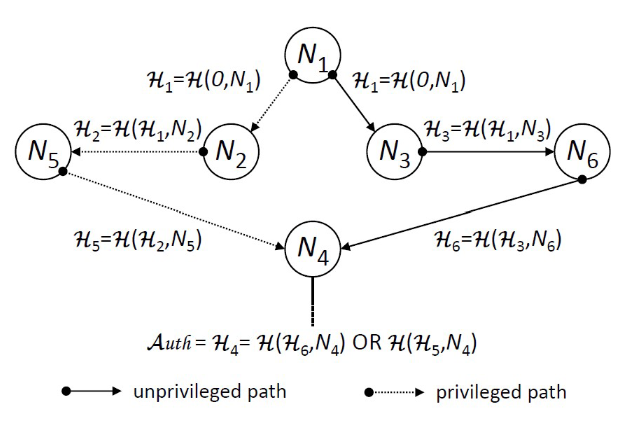
\includegraphics[scale=.5]{Figures/01/cflat.png}}
\caption{C-Flat}
\label{fig:c-flat}
\end{figure}

Lo-Fat\cite{dessoukyLOFATLowOverheadControl2017} is improving C-Flat by using hardware support for control flow attestation. Lo-Fat offline program analysis is still inheriting C-Flat approach.

Atrium \cite{zeitouniATRIUMRuntimeAttestation2017} is remote attestation scheme that can provide resiliency against physical memory attack where adversaries can exploit the property of Time of Check Time of Use (TOCTOU) during attestation. In this paper author are describing memory bank attack where adversary can control instruction fetches to benign memory area when attestation is running and direct the fetch to the malicious area otherwise.

\begin{figure}[htbp]
\centerline{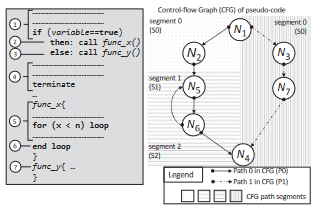
\includegraphics[scale=.5]{Figures/01/atrium.png}}
\caption{Atrium}
\label{fig:atrium}
\end{figure}

The offline measurement are calculated slightly different compared with C-Flat and Lo-Fat. In Atrium, the verifier perform one-time pre-processing to generate CFG of the program and computes cryptographic hash measurement over the instructions and addresses of basic blocks. C-Flat are only hash the node ID. While this approach can mitigate the TOCTOU attack, the offline measurement generation still grow exponentially as the complexity of the program grow. 

LiteHax \cite{dessoukyLiteHAXLightweightHardwareassisted2018} is hardware assisted remote attestation scheme that allow verifier to detect these different attacks:

\begin{itemize}
    \item control-data attack such as code injection or code reuse attack like ROP
    \item non-control-data attack
    \item data-only attack such us DOP which do not affect control flow
\end{itemize}

Different with the previous remote attestation scheme, the offline measurement phase of LiteHax are only generates program CFG without calculating any hash over all control flow and data flow events. However, in the online prover-side verification time, prover are still computing hash and sending it as report to the verifier. Verifier runs symbolic execution and incremental forward data-flow analysis without doing any lookup to offline measurement database.

Diat \cite{aberaDIATDataIntegrity2019} is remote attestation scheme that can attest data integrity and control-flow of autonomous systems. To improve efficiency of attestation, the program attested must be decomposed into small interacting modules. Data-flow monitoring is to be setup between critical modules. Control path attestation is being done against novel execution path representation using multiset has (MSH) function \cite{clarkeIncrementalMultisetHash2003}. The use of MSH makes some execution order of the program lost.

\begin{figure}[htbp]
\centerline{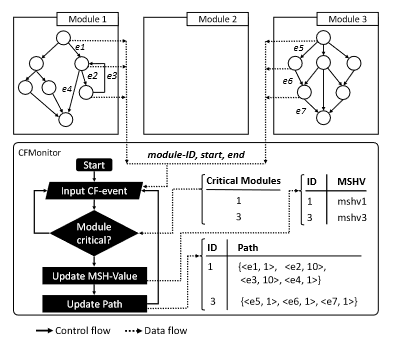
\includegraphics[scale=.5]{Figures/01/diat.png}}
\caption{Diat}
\label{fig:diat}
\end{figure}

OAT \cite{sunOATAttestingOperation2020} is remote attestation scheme to attest operation integrity of embedded device. OAT defines two type of measurements for control flow attestation: a trace (for recording branches and jumps) and a hash (for encoding returns). These two measurements are encoded as $H = Hash(H \bigoplus RetAddr)$ which called as attestation blob.

\begin{figure}[htbp]
\centerline{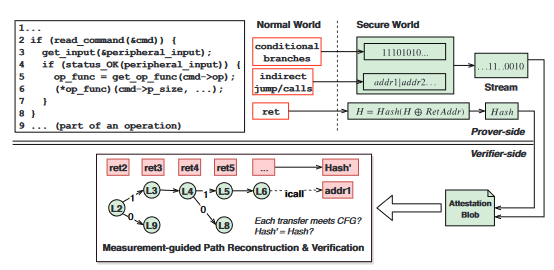
\includegraphics[scale=.5]{Figures/01/oat.png}}
\caption{OAT}
\label{fig:oat}
\end{figure}

During verification, verifier reconstruct paths from the attestation blob. The control flow violation is identified when CFI check against an address is failed or mismatched between hash and trace.

Although OAT does not encounter the combinatorial hash explosion in C-Flat, there is a verification overhead since verifier needs to reconstruct the attestation blob. TODO compare the overhead with ScaRR.

% Chapter 2

\chapter{Scope} % Main chapter title
\label{Chapter2} % For referencing the chapter elsewhere, use \ref{Chapter2} 

This chapter presents the scope of the thesis. Apart of literature review, the
main work on this research are the work on the models implementation for runtime
remote attestation and the analysis of the model's performance. Section
\ref{sec:implementation} presents the scope of implementation. Section
\ref{sec:analysis} discusses the scope of the analysis.

\section{Implementation}
\label{sec:implementation}

\begin{figure}[htbp]
\centerline{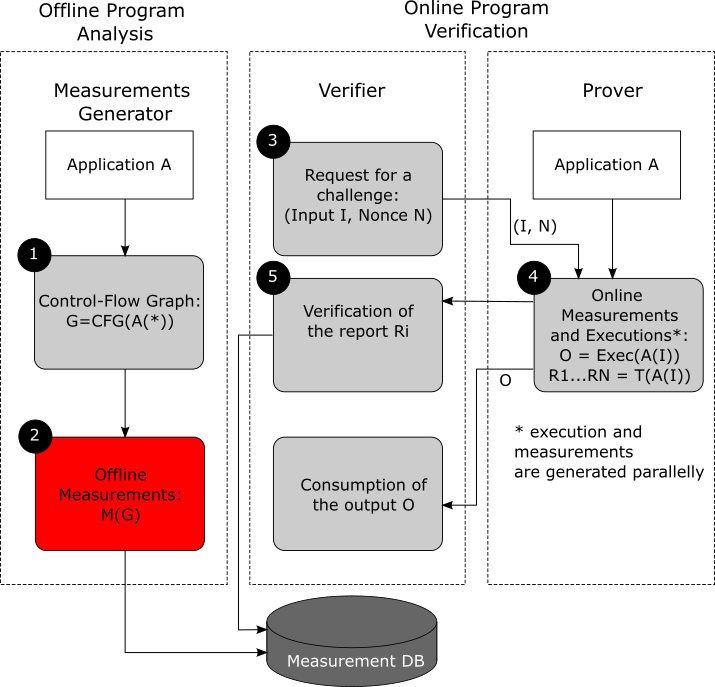
\includegraphics[scale=.5]{Figures/02/scarr-system-overview.png}}
\caption{ScaRR System Overview}
\label{fig:scarr-system-overview}
\end{figure}

In Chapter \ref{Chapter1}, we presented different runtime remote attestation
approaches. In learning the different models of runtime remote attestation, we
implemented one of the model: ScaRR Control-Flow Model
\cite{toffaliniScaRRScalableRuntime2019}. Specifically we write a tool to
extract offline measurement using the ScaRR control-flow model. ScaRR system as
shown in figure \ref{fig:scarr-system-overview}, consists of offline program
analysis and online program verification. This thesis will focus on the offline
program analysis part, specifically on the offline measurements generator as
shown in the red box in the figure \ref{fig:scarr-system-overview}.

The offline measurement is information that will be used in runtime remote
attesttion. We write the offline measurement as LLVM passes
\cite{lattnerLLVMINFRASTRUCTUREMULTISTAGE2002} using LLVM 13.0.0. We designed
the algorithm based on the description in the original paper. 

We tested the model implementation using different programs that is written in
C. Since the LLVM pass is running against the intermediate representation (IR),
we should get consistent result on any programming language that compiles to IR.

\section{Analysis}
\label{sec:analysis}

We analyze the control-flow model extracted against different programs with
various size and complexities. In this thesis, we are only analyzing program
written in C. The analysis is comparing the program size with different
measurements defined by the ScaRR control-flow model. We present the detail of
the methodology in chapter \ref{Chapter4} and show the analysis result in
chapter \ref{Chapter5}. 
% Chapter 3

\chapter{Background} % Main chapter title

\label{Chapter3} % For referencing the chapter elsewhere, use \ref{Chapter3} 

In this chapter, we start to present brief history of memory attacks and some background information on control-flow attack in section \ref{sec:control-flow-attack}. In section \ref{sec:remote-attestation}, we discuss how remote attestation helps to detect control-flow attack. We present ScaRR control flow model in section \ref{sec:scarr-model}. The chapter ends in section \ref{sec:llvm}, which share an overview of LLVM that relevant to the research. 

\section{Control Flow Attack}
\label{sec:control-flow-attack}

Control-flow attack happens when adversaries make a program to perform action of their choice without statically modify the program binary but alter the runtime properties of the program. The adversary intention can be to execute malicious operations or to leak secret information. Many of this runtime software security attacks are occured due to memory corruption bug in software written in low-level languages like C and C++ \cite{szekeresSoKEternalWar2013}.

Once memory corruption is triggered, there are different exploit types which adversary can use to perform the attack. Some of the relevant exploits are control-flow hijack \cite{shachamGeometryInnocentFlesh2007, schusterCounterfeitObjectorientedProgramming2015}  and data only attack \cite{chenNonControlDataAttacksAre2005, carliniControlFlowBendingEffectiveness2015}. 

Control-flow hijack can be classified further into code injection attack and code reuse attack such as return oriented programming \cite{roemerReturnorientedProgrammingSystems2012}.  Code injection attack will inject code in the program which will execute action prepared by the attacker. Code injection attack is already mitigated by solution like non-executable stack (NX), Data Execution Prevention and \( W \bigoplus R \) \cite{vanderveenMemoryErrorsPresent2012}. Code reuse attack will execute malicous action without injecting any codes, hence can't be detected by previosly mentioned defenses mechanism. As example, return-oriented program chains together short instruction sequences already present in a program’s address space, each of which ends in a \texttt{return} instruction. Unfortunately, ROP can not be mitigated by \( W \bigoplus R \) \cite{roemerReturnorientedProgrammingSystems2012}.

Memory error attacks and defenses have been always a continuous battle which unfortunately has not shown that it is over. In 2016, Abera et al proposed to use remote attestation to detect control flow attack \cite{aberaCFLATControlFlowAttestation2016}. 
That paper opened many researches in this area which we briefly presented in Chapter \ref{Chapter1}.
 
\section{Remote Attestation}
\label{sec:remote-attestation}

In this thesis we explore the use of remote attestation in detecting control-flow attack. Remote attestation is the activity of making a claim about properties of a remote target by supplying evidence to an appraiser over a network \cite{cokerPrinciplesRemoteAttestation2011a}. The ubiquitous deployment of IoT and different applications in the cloud require robust remote attestation method to ensure detection when the application is attacked.  Remote attestation scope was only covering static attestation of the application binary. However, in the recent years there have been more sophisticated attack that can alter the behavior of application so that static attestation does not suffice. 

In remote attestation, there are two roles involved, a trusted prover and a verifier. A prover is the one that must prove that the software has not been compromised. Verifier checks prover to ask the current state of runtime of the program. Alternatively, prover also can just update verifier periodically without being asked. The verifier compares the response from prover with the local database which has been generated before. If any of measurement mismatches, it means the has been violation due to an adversary's attack.

This research mainly focuses on offline measurement data generation for remote attestation which is used by verifier to validate the control flow graph. In the next section we discuss the detail of the control-flow model. We use LLVM in implementing the offline program analyzer.

\section{ScaRR Control-Flow Model} 
\label{sec:scarr-model}

ScaRR \cite{toffaliniScaRRScalableRuntime2019} are taking lesson learned from many former runtime remote attestation scheme to build model that can perform in a scalable way and can perform remote attestation on complex system. ScaRR control-flow model consists of two main components, checkpoint and list of action. 

As many previous runtime attestation scheme, ScaRR models and validates the attestion based on program's control flow graph. We need to run one-time measurement computation to extract checkpoints and list of actions of the program.

\subsection{Checkpoints} \label{sec:scarr-checkpoints}
Checkpoint is basic block of the program that delimit execution path of the program. ScaRR defines these different checkpoint types:
\begin{itemize}
    \item Thread Beginning: demarcating the start of program/thread
    \item Thread End: demarcating the end of program/thread
    \item Exit Point: representing exit point from application such as system call or out of translation unit function/library call
    \item Virtual-Checkpoint: managing cases for loop or recursion
\end{itemize}

In a program there should be at least Thread Beginning and Thread End checkpoints. Later depends on the structure of the program different checkpoint is marked in the program CFG.

\subsection{List of Actions}

List of actions (LoA) are edges (marked by two checkpoints) that direct one checkpoint to the next one. In program execution path, we only consider edges that identify the unique execution path.

LoA is defined through the following notation:


$$[(BBL_{s1},BBL_{d1}),...,(BBL_{sn},BBL_{dn})]$$

Consider again the CFG in the Figure \ref{fig:simple-loop-checkpoints}. The LoA between node 3 (Checkpoint Virtual) and node 10 (checkpoint ThreadEnd) is  $[(BBL_3, BBL_{10})]$. However, the LoA between node 0 and node 3 is $[]$ (empty set).


\section{LLVM}
\label{sec:llvm}

LLVM is compiler framework that was developed by Chris Lattner which provides portable program representation and different tooling. LLVM supports the implementation of different frontend, backend and middle optimizer for various programming languages \cite{lattnerLLVMCompilationFramework2004a}. 

\subsection{Intermediate Representation}

LLVM intermediate representation (IR) provides high-level information about programs to support sophisticated analysis and transformations. However, the representation is low-level enough to represent arbitrary programs and to allow extensive optimization. As an example, consider a simple C program in listing \ref{listing:sample-c}.

\begin{listing}[htbp]
    \inputminted[
    frame=lines,
    framesep=2mm,
    baselinestretch=1.2,
    fontsize=\footnotesize,
    linenos
    ]{c}{Code/03/sample.c}
    \caption{Simple C Program}    
    \label{listing:sample-c}
\end{listing}

The IR of the program can be seen in listing \ref{listing:sample-ll}. The text representation below, is just one of form of IR. Beside this readable instruction representation, LLVM IR also can be represented as byte code and in memory representation. In the IR, each line contains LLVM instructions. Instructions are grouped in basic blocks: container for instructions that execute sequentially. This arrangement, makes application control flow graph (CFG) to be explicit in the IR. The details of LLVM IR is available in the Language Reference \cite{LLVMLanguageReferencea}.

\begin{listing}[htbp]
    \inputminted[
    frame=lines,
    framesep=2mm,
    baselinestretch=1.2,
    fontsize=\footnotesize,
    linenos
    ]{llvm}{Code/03/sample.ll}
    \caption{LLVM IR The Sample C Program}    
    \label{listing:sample-ll}
\end{listing}


\begin{figure}[htbp]
\centerline{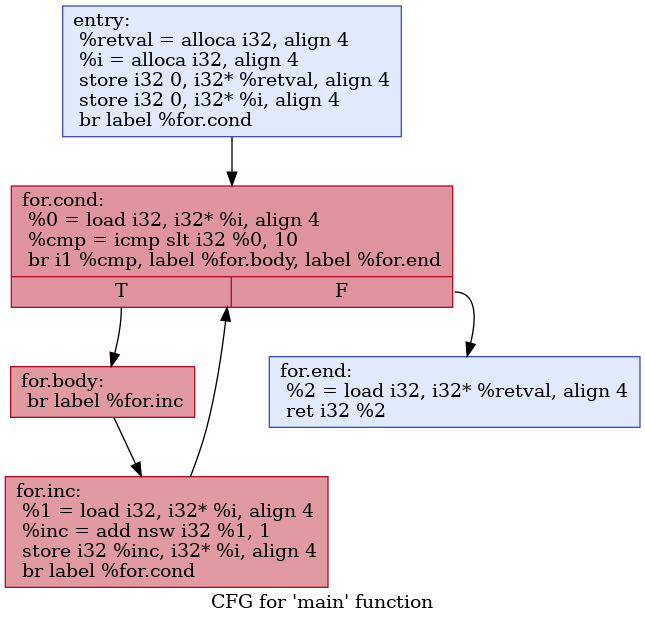
\includegraphics[scale=.5]{Figures/03/cfg.png}}
\caption{CFG for Simple C Program}
\label{fig:cfg}
\end{figure}


LLVM optimizer \textemdash{} which includes Analyzer and Transformer \textemdash{} are working on IR. In this thesis we are using this analyzer and transformer in building the Offline Program Analyzer.

\begin{figure}[htbp] 
    \centerline{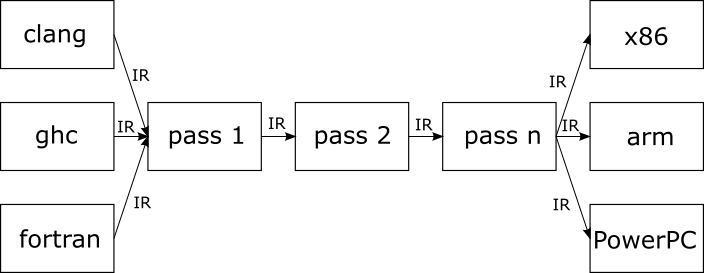
\includegraphics[scale=.75]{Figures/03/llvm-overview.png}} 
    \caption{LLVM Pass} 
    \label{fig:llvm} 
\end{figure} 

\subsection{LLVM Pass}

LLVM are applying transformations \textemdash{} which may include some analysis pipelines \textemdash{} and optimizations on tools called \texttt{opt}. \texttt{opt} is taking LLVM IR (either as text, bytecode or in memory) as input and then do transformations, analysis and optimizations on it (see figure \ref{fig:llvm}). Transformation and optimization alters the LLVM structure. Analysis gets information from the structure, which usually to be used by one or more transformations. Different transformations, optimizations and analyses are performed as pipelines of LLVM passes. LLVM pass can run per function, module or loop. LLVM function pass is executed once for every function in the program. LLVM module pass is executed once for every module. LLVM loop pass runs a time for each loop.  


In LLVM there are two ways of implementing Pass. First is using legacy approach and the latest one is using new pass manager approach. The approach different in structuring the code the implement the pass and also the way we use the pass.  In the legacy approach, we need to inherit from either \texttt{ModulePass}, \texttt{FunctionPass} or \texttt{LoopPass} and override \texttt{runOnXXX} method (xxx is either Function, Module or Loop). In the newer approach we have to inherit CRTP mix-in \texttt{PassInfoMixin<PassT>} and override the run method.

The way we use the pass, in legacy approach we need to provide the pass name as literal argument to \texttt{opt}. See the example in listing \ref{listing:legacy-llvm-pass}. In the new pass manager, we are putting the pass name after `--passes` argument in comma separated list (listing \ref{listing:new-llvm-pass}). The pass is executed in order.

\begin{listing}[htbp]
    \begin{minted}[
        frame=lines,
        framesep=2mm,
        baselinestretch=1.2,
        fontsize=\footnotesize,
        ]{bash}
        opt --dot-cfg file.ll 
    \end{minted}
    \caption{Running Legacy LLVM Pass}    
    \label{listing:legacy-llvm-pass}
\end{listing}

\begin{listing}[htpb]
    \begin{minted}[
        frame=lines,
        framesep=2mm,
        baselinestretch=1.2,
        fontsize=\footnotesize,
        ]{bash}
        opt -passes=scarr-cp-marker,scarr-loa-collector file.ll 
    \end{minted}
\caption{Running LLVM New Pass}    
\label{listing:new-llvm-pass}
\end{listing}

\subsection{LLVM API}

In writing LLVM pass, we use LLVM API. In this section we present relevant component that is required in implementing LLVM Pass for the Offline Program Analyzer. LLVM API is leveraging many C++ features and libraries such as template and STL. The API also provides many ready to use data structure which is not available in the STL. A more broad discussion on the important element of the API is available in the Programmers Manual \cite{LLVMProgrammerManuala}. Complete API documentation can be referred at the doxygen page \cite{LLVMLLVMa}.

\subsubsection{Module}

Module is the top level container for all other IR objects. Module contains list of global variables, functions, symbol tables and other various data about target characteristics. Module can be a single translation unit of a program (source file) or can be multiple translation unit combined by linker. 

In LLVM pass, we can get access to module by implementing a Module pass or by parsing IR using \texttt{parseIR} or \texttt{parseIRFile} from \texttt{IRReader.h}. Once we get a handler to a module, getting a functions within module is as simple as passing module to a loop, since module provides iterator that return list of function in the module (see listing \ref{listing:llvm-module-api}).

\begin{listing}[htbp]
    \inputminted[
        frame=lines,
        framesep=2mm,
        baselinestretch=1.2,
        fontsize=\footnotesize,
        linenos
    ]{cpp}{Code/03/module.cpp}
    \caption{LLVM Module API}    
    \label{listing:llvm-module-api}
\end{listing}

\subsubsection{Function}

Function in LLVM represents function in the source program. A function contains list of zero or more BasicBlocks. There is one entry BasicBlock and can be multiple exit BasicBlocks. We can get handler to a function either by getting the iterator from a module instance or by implement a Function Pass. By using optimization, syntax hint or using an inliner pass, a function can be inlined. In this thesis, we are using \emph{inliner-wrapper} pass to inline most function before feeding the IR into the ScaRR passes.

\subsubsection{Basic Block}

Basic Block represents single entry and single exit section of the code. The single exit can be one of terminator instruction — branches, return, unwind and invoke. We can get handle to a basic block from function. Refer to listing \ref{listing:llvm-basic-block-api} to see how to get the basic block.

\begin{listing}[htbp]
    \begin{minted}[
        frame=lines,
        framesep=2mm,
        baselinestretch=1.2,
        fontsize=\footnotesize,
        linenos
    ]{cpp}
        for (auto &function: *module) {
            for (auto &basicBlok: function) {
                // do thing with Basic Block
            }
        }
    \end{minted}
    \caption{LLVM Basic Block API}    
    \label{listing:llvm-basic-block-api}
\end{listing}

\subsubsection{Graph Traversal}

Since LLVM CFG is already structured as a graph, the basic block can be traversed using different ready to use graph traversal algorithm. LLVM offers some common graph traversal algorithms such as breadth first search and depth first search. The algorithms can be used immediately on basic blocks and functions. If there is a need to traverse a custom structure, the algorithms just require the new structure to implement \emph{GraphWriter} interface.

\subsection{Tools}

We are implementing the algorithms using different tools. We are highlighting some of those in this section so that everyone interested can replicate the step.

\subsubsection{clang}

\texttt{clang} is one of the frontend provided by LLVM. It can compiles C, C++ and Objective C. \texttt{clang} command line arguments are compatible with widely use gcc compiler. The main use of \texttt{clang} in this research is to compile source files into LLVM IR text files. Listing \ref{listing:compile-llvm-to-ir} shows how to compile a C program into LLVM IR. 

\begin{listing}[htbp]
    \begin{minted}[
        frame=lines,
        framesep=2mm,
        baselinestretch=1.2,
        fontsize=\footnotesize,
    ]{bash}
        clang -S -emit-llvm source.c
    \end{minted}
    \caption{Compiling C to LLVM IR}    
    \label{listing:compile-llvm-to-ir}
\end{listing}
    
We can pass optimization level from 0 (no-optimization) to 3 (most optimal, can make code run faster but larger in size) when compiling the source code.

By default, clang strips out value names and do some optimization when generating LLVM IR. We can use this flag to disable optimization and get readable value names that can help when troubleshooting and exploring the generated IR. Listing \ref{listing:compile-llvm-to-ir-no-opt} shows how to compile to IR without any optimization and to preserve the function and variable names.

\begin{listing}[htbp]
    \begin{minted}[
        frame=lines,
        framesep=2mm,
        baselinestretch=1.2,
        fontsize=\footnotesize,
    ]{bash}
        clang -S -emit-llvm -Xclang -disable-O0-optnone \
        -fno-discard-value-names source.c
    \end{minted}
    \caption{Compiling C to LLVM IR without Optimization}    
    \label{listing:compile-llvm-to-ir-no-opt}
\end{listing}

\subsubsection{opt}

\texttt{opt} is LLVM optimizer and analyzer that can be invoked from command line. We are using \texttt{opt} to execute the offline program analyzer which marks basic block checkpoints and calculate list of action which can be used as information to detect control flow violation during remote attestation.

\subsubsection{cmake}

\texttt{cmake} is a build file generator which is have an important role in large project like LLVM. Although the deep understanding of \texttt{cmake} is not required in implementing LLVM pass, but we need to know at least how to build the pass after the implementation so that we can run it.

LLVM can be downloaded using git. See Listing \ref{listing:clone-llvm-code}. This thesis is implemented on LLVM 13.0.0.

\begin{listing}[htbp]
    \begin{minted}[
        frame=lines,
        framesep=2mm,
        baselinestretch=1.2,
        fontsize=\footnotesize,
    ]{bash}
        git clone https://github.com/llvm/llvm-project
    \end{minted}
    \caption{Cloning LLVM Source Code}    
    \label{listing:clone-llvm-code}
\end{listing}

Once it is downloaded we can go to the LLVM directory and generate the build files. \texttt{cmake} supports several build tools such as make and ninja. Refer to listing \ref{listing:build-llvm}.

\begin{listing}[htbp]
    \begin{minted}[
        frame=lines,
        framesep=2mm,
        baselinestretch=1.2,
        fontsize=\footnotesize,
        linenos
    ]{bash}
        cd llvm-project/llvm
        mkdir build
        cd build
        cmake -G Ninja ../ # generate build file for Ninja
        ninja opt # build only opt
    \end{minted}
\caption{Building LLVM}    
\label{listing:build-llvm}
\end{listing}

With all background discussion in this chapter we should be ready to discuss the methodology in Chapter \ref{Chapter4}.
% Chapter 4

\chapter{Methodology} % Main chapter title

\label{Chapter4} % For referencing the chapter elsewhere, use \ref{Chapter4} 

In this chapter, we present the methodology of the research. First we present 
the threat model. \ft{same as before, add reference to the subsections}
After that, we show the overview of the implementation of the 
ScaRR algorithm to extract checkpoint and list of action. The section about 
ScaRR control-flow model will follow. The last two section is the detail on 
LLVM implementation to get checkpoints and list of actions from codes. 
Checkpoints and list of actions are collected to build offline measurement 
database that is used for the remote attestation.

\section{Threat Model}

The threat model in this research is taken from ScaRR
\cite{toffaliniScaRRScalableRuntime2019}. There are two parties: attacker and 
prover. The attacker has aim to hijact the application control flow by using 
various memory attacks described in Chapter \ref{Chapter3}.
\ft{add some example here too, moreover, ScaRR considers any attacker in 
user-space, not only code-reuse attacks.}
Moreover, we do not consider physical attack and data-oriented attack which 
does not alter program CFG.
The prover uses kernel as trusted anchor and has common memory corruption 
attack mitigations such as \( W \bigoplus R \) and ASLR. 
\ft{moreover, split attacker and defender capabilities in two paragraphs. Like:}

\vspace{0.5cm}
\noindent \textbf{Attacker capabilities:}
The attacker can do this, that, and this other..

\vspace{0.5cm}
\noindent \textbf{Defender capabilities:}
We assume the defender is a white knight without fear! Arming a spear and 
fighting the dragon.

\ft{ok, I don't ensure the aforementioned information is correct..}

\section{Overview of The Offline Measurement}\
\label{sec:overview}

The goal of the offline measurement is to get the information to be used in the 
remote attestation. In this research we implement ScaRR Control-flow model 
\cite{toffaliniScaRRScalableRuntime2019} which we also elaborate in the Section 
\ref{sec:scarr-model}. These are the steps that we do in getting the offline 
measurements:

\ft{make a picture that shows three blocks from left to right. Then, describe 
the three parts briefly and point them to their dedicated section below.}

\begin{enumerate}
    \item Flattenning the CFG
    \item Marking the Checkpoints
    \item Finding the List of Actions
\end{enumerate}

\begin{listing}[htbp]
    \begin{minted}[
        frame=lines,
        framesep=2mm,
        baselinestretch=1.2,
        fontsize=\footnotesize
        ]{c++}
        int main() {
            for (int i = 0; i < 10; i++) {
                // do nothing
            }
        }
    \end{minted}
    \caption{Simple Loop}    
    \label{listing:simple-loop}
\end{listing}

\subsection{Flattenning the CFG}

\ft{sorry dear but this part is not clear. you should start: why do we need 
flatting? what flattening means? can you give an example? add a listing (simple 
one) with a main calling the same function A twice, thus show the graph before 
and after flatting. For the CFG, you can just drawn, no need to extract it from 
LLVM Pass. If not clear, we better talk.}

Consider the program in listing \ref{listing:simple-loop}. The CFG is shown in the figure \ref{fig:simple-loop-cfg}. The first step of the offline measurement is to flatten the CFG to get all the basic block list. We can flatten the CFG into basic block with one out of some graph traversal algorithm in LLVM. The CFG in figure \ref{fig:simple-loop-cfg} contains these following basic blocks:

\begin{itemize}
    \item Basic Block \%0
    \item Basic Block \%3
    \item Basic Block \%6
    \item Basic Block \%7
    \item Basic Block \%10
\end{itemize}


\begin{figure}[htbp]
\centerline{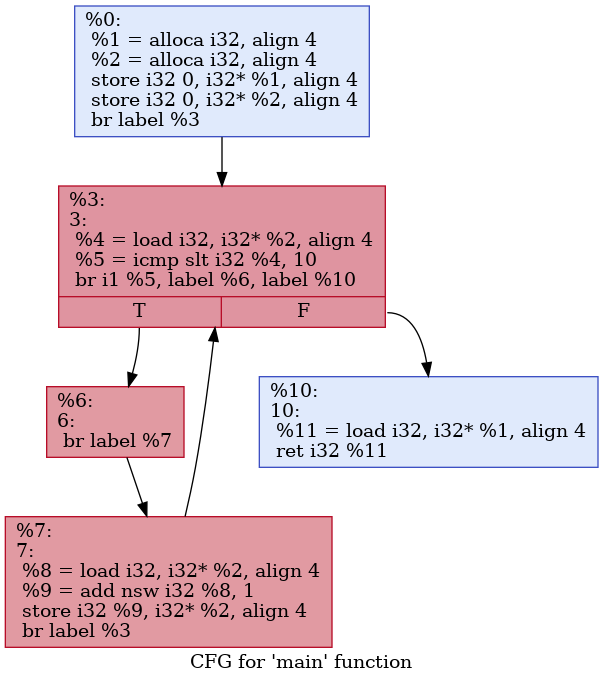
\includegraphics[scale=.5]{Figures/04/simple-loop.png}}
\caption{Simple Loop CFG}
\label{fig:simple-loop-cfg}
\end{figure}

\subsection{Marking the Checkpoints}


After we flatten CFG into basic block, we will check each of basic block to 
find different kind of checkpoints. The marked checkpoints from the CFG in 
Figure \ref{fig:simple-loop-cfg} can be seen in Figure 
\ref{fig:simple-loop-checkpoints}.

\ft{expand this part by a lot! what are the checkpoints? which heiristics use 
to identify them? virtual checkpoints from loops? start? discuss better. Also, 
for each heuristics, you should add a specific paragraph (as in the threat 
model)}

\begin{figure}[htbp]
\centerline{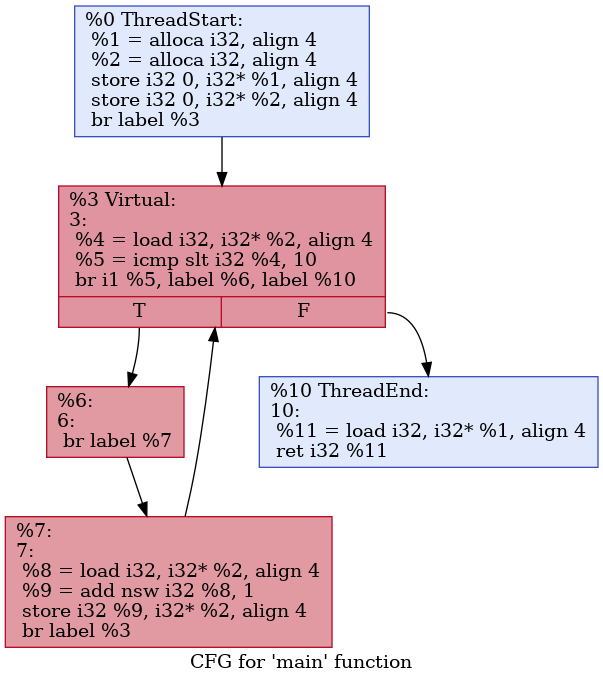
\includegraphics[scale=.5]{Figures/04/simple-loop-checkpoints.png}}
\caption{Loop CFG}
\label{fig:simple-loop-checkpoints}
\end{figure}

\subsection{Finding the List of Actions}

The step of finding LoA is traversing path between two checkpoints and add significant basic block that traverse the path between the two checkpoints. The detail of this step is explained in the next sections.

\section{ScaRR Control-Flow Model} \label{sec:scarr-model}

\ft{move this in background. You can say that you focus on ScaRR cfg model 
because is part of the thesis, or something like this.
Rule-of-thumb, add a label to a section/subsection as soon you make it.}

ScaRR \cite{toffaliniScaRRScalableRuntime2019} are taking lesson learned from many former runtime remote attestation scheme to build model that can perform in a scalable way and can perform remote attestation on complex system. ScaRR control-flow model consists of two main components, checkpoint and list of action. 

As many previous runtime attestation scheme, ScaRR models and validates the attestion based on program's control flow graph. We need to run one-time measurement computation to extract checkpoints and list of actions of the program.

\subsection{Checkpoints} \label{sec:scarr-checkpoints}
Checkpoint is basic block of the program that delimit execution path of the program. ScaRR defines these different checkpoint types:
\begin{itemize}
    \item Thread Beginning: demarcating the start of program/thread
    \item Thread End: demarcating the end of program/thread
    \item Exit Point: representing exit point from application such as system call or out of translation unit function/library call
    \item Virtual-Checkpoint: managing cases for loop or recursion
\end{itemize}

In a program there should be at least Thread Beginning and Thread End checkpoints. Later depends on the structure of the program different checkpoint is marked in the program CFG.

\subsection{List of Actions}

List of actions (LoA) are edges (marked by two checkpoints) that direct one checkpoint to the next one. In program execution path, we only consider edges that identify the unique execution path.

LoA is defined through the following notation:

$$[(BBL_{s1},BBL_{d1}),...,(BBL_{sn},BBL_{dn})]$$

Consider again the CFG in the Figure \ref{fig:simple-loop-checkpoints}. The LoA between node 3 (Checkpoint Virtual) and node 10 (checkpoint ThreadEnd) is  $[(BBL_3, BBL_{10})]$. However, the LoA between node 0 and node 3 is $[]$ (empty set).

\section{ScaRR LLVM Pass} 

\ft{no need this section. Consider your main section is overview 
(Sec~\ref{sec:overview}), all the rest should revolve around it. If you want to 
add a link ti your pass, you can do it in the result.}
ScaRR LLVM pass\footnote{https://github.com/lamida/llvm-project/pull/3} is the implementation of ScaRR offline measurement using LLVM. ScaRR offline measurement is represented as the following key-value pair.

$$(cp_A, cp_B, H(LoA)) \Rightarrow [(BBL_{s1}, BBL_{d1}), ..., (BBL_{sn}, BBL_{dn})]$$

As described in the section \ref{sec:scarr-checkpoints}, checkpoint is a special basic block that delimit path between execution path in a CFG. $cp_A$ is the start delimiter of the path. $cp_B$ is the end of delimiter. $LoA$ — list of action — is list of significant basic block pairs which define edges 

ScaRR extractor traverses the graph in two passes. The first pass is find whether the basic block is a checkpoint (section \ref{sec:scarr-checkpoint-marker}). The second pass traverses the graph and mark List of Action between every two checkpoint (section \ref{sec:scarr-loa-collector}). 

\section{ScaRR Checkpoint Marker} \label{sec:scarr-checkpoint-marker}

\ft{in fact! this part shoudl be used before :) where you describe the 
checkpoints. I, as a reader, expect you exaust the discussion about checkpoints 
before, why 2 sections that say the same things?}
The logic of checkpoint marker is to traverse the whole control flow graph at least once. For each basic block, we have to check whether the basic block can be considered as any of checkpoint type mentioned above. To allow marking additional information about ScaRR checkpoint, we are modifying the BasicBlock class to add checkpoint instance variable as shown in listing \ref{listing:checkpoint}.

\begin{listing}[htbp]
    \begin{minted}[
        frame=lines,
        framesep=2mm,
        baselinestretch=1.2,
        fontsize=\footnotesize,
        linenos
    ]{c++}
        class BasicBlock ... {
        private:
        // add checkpoint field
            Checkpoint cp;

        public:
            // setter and accessor
        void setCheckpoint(Checkpoint);
        Checkpoint getCheckpoint() const;
        ...
        }
    \end{minted}
    \caption{Add Checkpoint Instance Variable to BasicBlock class.}    
    \label{listing:checkpoint}
\end{listing}

The algorithm to mark the checkpoint is first we iterate all basic block in main function. First we mark the first basic block with no predecessor as ThreadStart checkpoint and basic block with no successor and ThreadEnd checkpoint. 

\ft{correct, I expect something like this, but not in this section, put 
altogether in the previous checkpoints subsection}
To identify ExitPoint checkpoint, for each basic block then we iterate  each instruction to find whether any instruction in the basic block is a `call` instruction and has no body defined in this translation unit. Please refer to Listing \ref{listing:exit-point-cp}.

\begin{listing}[htbp]
    \begin{minted}[
        frame=lines,
        framesep=2mm,
        baselinestretch=1.2,
        fontsize=\footnotesize,
        linenos
    ]{c++}
        for (auto &basicBlock: Function) {
            for (auto &instruction : basicBlock) {
                if (isa<CallInst>(i)) {
                auto *call = &cast<CallBase>(i);
                if (call != nullptr && call->getCalledFunction()->empty()) {
                    // this basicBlock is ExitPoint
                    basicBlock.setCheckpoint(Checkpoint::ExitPoint);
                } 
            }
        } 
    \end{minted}
    \caption{Finding ExitPoint Checkpoint}    
    \label{listing:exit-point-cp}
\end{listing}

To mark Virtual checkpoint, we need to find loop header basic block. Although there is no direct API to check whether a basic block is a loop header, LLVM provide it in LoopInfoBase API. See Listing \ref{listing:virtual-cp}

\begin{listing}[htbp]
    \begin{minted}[
        frame=lines,
        framesep=2mm,
        baselinestretch=1.2,
        fontsize=\footnotesize,
        linenos
    ]{c++}
        void findVirtualCheckpoint(DominatorTree &DT, Function &F) {
            DT.recalculate(F);
            // generate the LoopInfoBase for the current function
            LoopInfoBase<BasicBlock, Loop>* KLoop = new LoopInfoBase<BasicBlock, Loop>();
            KLoop->releaseMemory();
            KLoop->analyze(DT);
            for (auto &bb : F) {
                // Since the BasicBlock would have been inlined, just traverse from main function
                if (F.getName() == "main") {
                auto loop = KLoop->getLoopFor(&bb);
                if (loop != nullptr) {
                    // found VirtualCheckpoint
                            loop->getHeader()->setCheckpoint(Checkpoint::Virtual);
                }
                }
            }
        }
    \end{minted}
    \caption{Getting Virtual Checkpoint}
    \label{listing:virtual-cp}
\end{listing}

\section{ScaRR LoA Collector} \label{sec:scarr-loa-collector}

\ft{can you summarize the algorithm in a pseudocude fashion? you should link 
the lines in the pseudo code and describe it step by step.}

The algorithm of getting LoA between two checkpoints is little bit more complex. First, we iterate all the basic block and if the basic block is a checkpoint we mark this is $cpA$. Next, we recursively traverse the successor of $cpA$ until we find another checkpoint $cpB$. It is possible for $cpA = cpB$. If there is no branch between the two checkpoint, the LoA is an empty set. If there is a branch, the first LoA is always be $cpA$ and the second LoA is always be the first basic block after the branch \textemdash{} which can be $cpB$ or just non checkpoint basic block. Interested readers can refer to the implementation of this pass to see the detail.

\subsection{Running The Pass}

To mark the list of Checkpoints, we can invoke LLVM \texttt{opt} as shown in listing \ref{listing:mark-cp-in-cfg}.

\begin{listing}[htbp]
    \begin{minted}[
        frame=lines,
        framesep=2mm,
        baselinestretch=1.2,
        fontsize=\footnotesize,
    ]{c++}
        opt -passes=scarr-cp-marker <file>.ll
    \end{minted}
    \caption{Mark Checkpoint in BasicBlock}    
    \label{listing:mark-cp-in-cfg}
\end{listing}

We can see the basic blocks output that has been marked with checkpoint using LLVM dot-cfg pass.

\begin{listing}[htbp]
    \begin{minted}[
        frame=lines,
        framesep=2mm,
        baselinestretch=1.2,
        fontsize=\footnotesize,
    ]{c++}
        opt -passes=scarr-cp-marker,dot-cfg <file>.ll
    \end{minted}
    \caption{Print Checkpoints in CFG dot file}    
    \label{listing:cp-to-cfg}
\end{listing}

The commands in listing \ref{listing:cp-to-cfg} generates different dot files per function. We can use xdot command line from graphiz to see the graph. 

To mark the list of actions between checkpoints, we can invoke LLVM \texttt{opt} as shown in Listing \ref{listing:get-loa}

\begin{listing}
    \begin{minted}[
        frame=lines,
        framesep=2mm,
        baselinestretch=1.2,
        fontsize=\footnotesize,
    ]{c++}
        opt -passes=scarr-cp-marker,scarr-loa-collector <file>.ll
    \end{minted}
    \caption{Get List of Actions}    
    \label{listing:get-loa}
\end{listing}

Note that we have to run scarr-cp-marker before scarr-loa-collector.

The result and its interpretation are discussed in the next chapter. 
% Chapter 5

\chapter{Results} % Main chapter title

\label{Chapter5} % For referencing the chapter elsewhere, use \ref{Chapter5} 

In this research we used the offline measurement generator in getting the 
measurement across different real world programs. We calculate the ScaRR 
control flow information for each of the programs and we analyse and present the result in this chapter. 
The analysis and source code of the program is available in this Github repository: \url{https://github.com/lamida/scarr-sample-program/}.

In this research we choose 4 large open source projects for analysis. We download the source code and checkout the latest version of the code. 
The first software is Redis $6.2.4$  \cite{RedisRedis2021}, a what so called data structure server that is widely used in real world. 
The Redis source build consist of the server binary and the client cli. We analyse both of the program.

The second program we analyse is bzip2 $1.08$ \cite{Bzip2Bzip2}. Bzip2 is free and open source file compression program. The third program is openssl $1.1.1j$ \cite{OpensslOpenssl2021}. OpenSSL is full-featured toolkit for TLS protocol. 

The last suite program we analyse is coreutils $8.32$ \cite{CoreutilsCoreutils2021}. Coreutils is suite of Unix utilities for file, shell and text manipulation.

For each of program, we are collecting the following measurements:

\begin{itemize}
    \item source code lines
    \item IR lines
    \item number of basic blocks (nBB)
    \item number of ScaRR measurements (nM)
    \item number of checkpoints (nCP)
    \item number of LoA (nLoA)
\end{itemize}

\section{ScaRR Control Flow Result}

\xt{Elaborate the results, add charts for better visualization than just table.}
\xt{TODO: remove this long table and use simpler visualization}

\csvautolongtable{csv/coreutils.csv}
\xt{Find a way to add caption to this long table}

\begin{table}[hbtp]
    \centering
    \csvautotabular{csv/redis.csv}
    \caption{Redis ScaRR measurements}
\end{table}

\begin{table}[hbtp]
    \centering
    \csvautotabular{csv/misc.csv}
    \caption{Some additional programs ScaRR measurements}
\end{table}

\section{Complexity Analysis}

TBD

\section{Case Study}

TBD 
% Chapter 5

\chapter{Discussion and Future Works} % Main chapter title

\label{Chapter6} % For referencing the chapter elsewhere, use \ref{Chapter6} 

In Chapter~\ref{Chapter5}, we discuss the result of ScaRR's offline measurement
generator. We learn that the algorithm time complexity is linear to the input.
The input here is the size of the program. We measure the size of the program as
the size of source code lines. The number of lines is also linear with the size
of intermediate representation and basic blocks number. The most important
finding we confirm ss the number of measurements is also linear with the program
size. We know now that we can use the algorithm to do runtime remote attestation
for a complex program.

In this study, we identify the limitation of the algorithm. We can use the
findings for possible future works. First, we do not test the algorithm with a
program that contains recursion, signals, and exception. We also only test the
algorithm with a single-thread program. We only run the analysis on C programs.

We also noticed the limitation on the algorithm that cannot detect non-control
data attacks. Non-control data attack does not modify program CFG. Next, the
algorithm does not track the number of loop iteration. The algorithm does know
whether a program is going to a loop. Unfortunately, the algorithm does not know
how many iterations a program should run. The offline measurement cannot know
when there is an attack that modifies the number of the loop.  

%----------------------------------------------------------------------------------------
%	THESIS CONTENT - APPENDICES
%----------------------------------------------------------------------------------------

\appendix % Cue to tell LaTeX that the following "chapters" are Appendices

% Include the appendices of the thesis as separate files from the Appendices folder
% Uncomment the lines as you write the Appendices

% Appendix A

\chapter{Appendix Title Here} % Main appendix title

\label{AppendixA} % For referencing this appendix elsewhere, use \ref{AppendixA}

Write your Appendix content here.
%\include{Appendices/AppendixB}
%\include{Appendices/AppendixC}

%----------------------------------------------------------------------------------------
%	BIBLIOGRAPHY
%----------------------------------------------------------------------------------------

\printbibliography[heading=bibintoc]

%----------------------------------------------------------------------------------------

\end{document}  
